%%%%%%%%%%%%%%%%%%%%%%%%%%%%%%%%%%%%%%%%%%%%%%%%%%%%%%%%%%%%%%%%%%%%%%%%%%%%%%%
%%                                                    DATA SIMULATION SELECTION
%%%%%%%%%%%%%%%%%%%%%%%%%%%%%%%%%%%%%%%%%%%%%%%%%%%%%%%%%%%%%%%%%%%%%%%%%%%%%%%
%%                                    about the samples, MC Generation and cuts 



%______________________________________________________________________________
%                                                Daten Simulation und Selektion 
\chapter{Daten, Simulation \& Selektion}

\begin{quote}
    The abstract come last
\end{quote}



%______________________________________________________________________________
%                                                                         Daten 
\section{Daten}
\label{data_sim_selection:data}

\begin{itemize}
    \item \sout{Daten von 2012}
    \item \sout{Parameter: Energie, Bunchespacing, Perioden}
    \item HV-Problem Anfang des Jahres
\end{itemize}

Die Daten, die dieser Arbeit zugrunde liegen, wurden vom ATLAS-Detektor im Jahr
2012 bei erstmalig $8 \TeV$ Schwerpunktsenergie aufgenommen. Der \ac{LHC} wird
mit Paketen von Protonen, sogenannte Bunches (vom engl. Bunch: Bündel) gefüllt,
die für einige Stunden im Beschleuniger zirkulieren\footnote{weitere Details:
siehe Kapitel \ref{}}.
Eine solche Füllung steht für identische Einstellungen des Beschleunigers bzw.
Detektors und wird in ATLAS mit einer fortlaufenden Nummer identifiziert.
Die Füllungs-Nummern größerer Perioden konstanter Bedingungen, wie das zu der
Zeit implementierte Trigger-Menü oder globale \ac{LHC} Parameter, werden dann
mit einem Buchstaben zusammengefasst (Periode A, B, ...).

Der vorliegende Datensatz wurde in der Zeit zwischen dem 04. April 2012 und dem
16. Dezember 2012 aufgenommen und umfasst 10 Perioden, die einer integrierten
Gesamtluminosität von $20.3 \fb^{-1}$ entsprechen\footnote{nach Anwenung der
\ac{GRL} (siehe Kapitel \ref{})} (siehe Abbildung \ref{fig:lumi}). Der Detektor
wurde hierbei in einer Konfiguration betrieben, die einen zeitlichen Abstand
zwischen den Teilchen-Paketen von $50\:\nano\second$ gewährleistet, woraus eine
instantane Luminosität\footnote{Erläuterungen zur Messung der Luminosität in
ATLAS finden sich in Kapitel \ref{}} von bis zu
$7.73 \cdot 10^{-33} \centi\meter^{-2}\second^{-1}$ resultiert.

Eine hohe instantane Luminosität verspricht eine große Rate interessanter
Ereignisse, jedoch bedingt sie auch viele unerwünschte Neben-Ereignisse,
vorwiegend aus inelastischen Streuprozessen, die einen signifikanten Einfluss
auf die Messung nehmen können. Dieser Effekt wird als \textit{Pile-Up}
bezeichnet und ist in Abbildung \ref{fig:pileup} illustriert.

\begin{figure}
    \begin{minipage}[b]{0.48\textwidth}
        \centering
        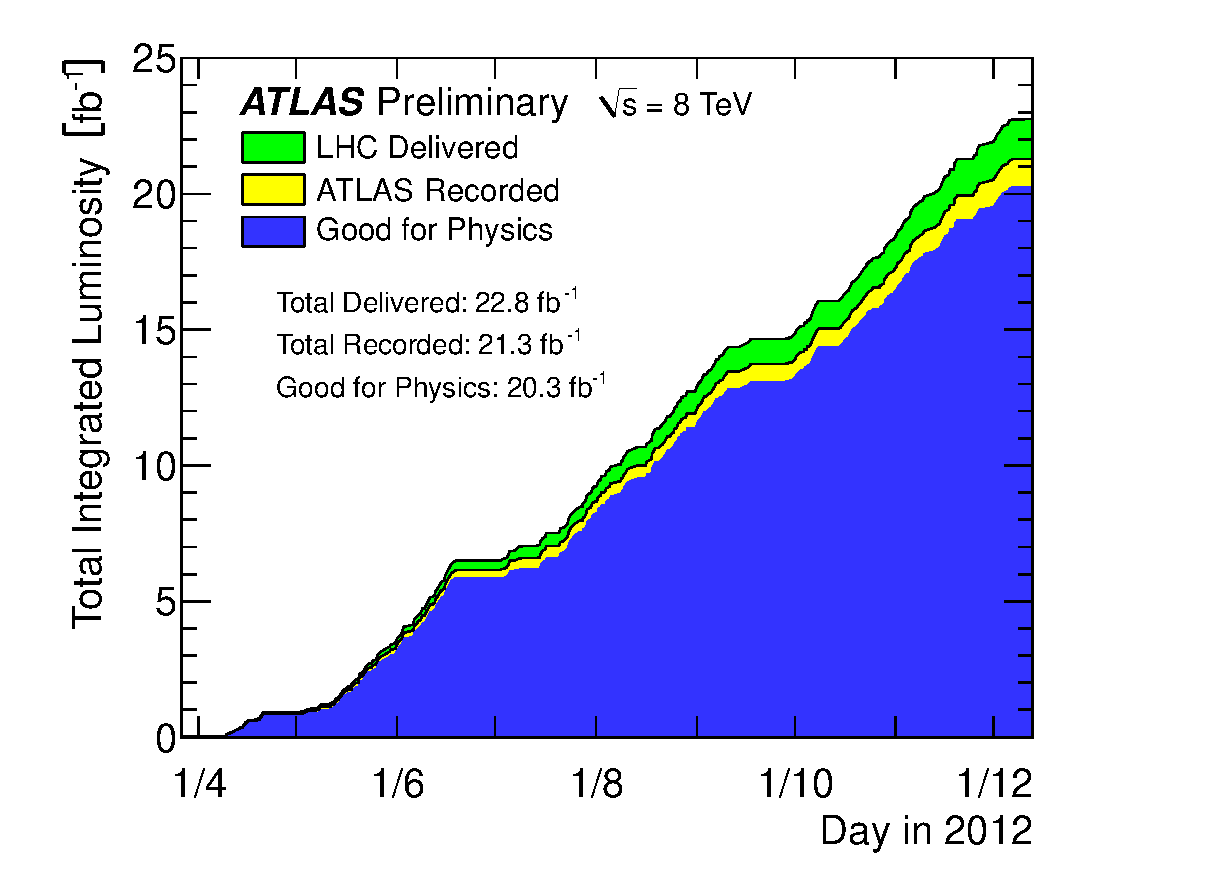
\includegraphics[width=1.\textwidth]{plots/lumi}
        \captionsetup{format=plain}
        \caption{Verfügbare, aufgezeichnete und validierte integrierte
            Luminosität aufgetragen gegen die Zeit innerhalb der Messkampange}
        \label{fig:lumi}
    \end{minipage}
    \hfill
    \begin{minipage}[b]{0.48\textwidth}
        \centering
        \includegraphics[width=1.\textwidth]{img/pileup}
        \captionsetup{format=plain}
        \caption{Ereignisse mit $Z \rightarrow \mu\mu$ Kandidat und hohem
            Pile-Up. 25 rekonstruierte Vertizes.}
        \label{fig:pileup}
    \end{minipage}
\end{figure}

HV-Problem \development



%______________________________________________________________________________
%                                                                    Simulation
\section{Simulation}
\label{data_sim_selection:simulation}

\begin{itemize}
    \item \sout{Motivation für Simulation (Theorie-Vorhersage)}
    \item \sout{Mehrschrittiges Prinzip}
    \item \sout{Eventgeneration (Matrixelemente, Fragmentation,...)}
    \item \sout{Detektorsimulation (+ Ausgabeformat)}
    \item \sout{Nötige Korrekturen (Pileup, Effizienzen, Smearing, kFaktors)}
    \item Übersicht und kurze(!) Statements zu Samples
    \item LumiScaling
\end{itemize}

Die Simulation von Ereignissen und des Detektors ist ein wichtiger Bestandteil
von Analysen in der Hochernergiephysik. Sie repräsentiert einerseits das
beste Wissen über die betrachteten Prozesse und die genaue Kenntnis des
Detektors, andererseits lassen sich mit Simulationen die Erweiterungen durch
neue theoretische Modelle untersuchen und deren Einfluss auf bereits bekannte
Prozesse vorhersagen. Zentraler Gegenstand der Betrachtung ist hierbei stets
der Vergleich zwischen Simulation und realen Daten.



\subsection{Erzeugung simulierter Datensätze}
\label{event_generation}
Die Erstellung einer Simulation geschieht für gewöhnlich in mehreren Schritten.
Eine grobe Unterteilung ist die Unterscheidung zwischen der Simulation des
eigentlichen physikalischen Prozesses, wie beispielsweise die Annihilation
eines Quarks und eines Antiquarks zu einem Z-Boson und dessen nachfolgenden
Zerfall in ein Leptonpaar, und die Simulation der Detektorantwort, also der
Betrachtung aller physikalischer Subprozesse, die von den Produkt-Teilchen im
Detektor induziert werden (Detektor-Antwort).

Im ersten Schritt, der Ereignis-Simulation, kommen so genannte
\textit{Monte-Carlo Generatoren} zum Einsatz. Dies sind meist von theoretischen
Physikern implementierte Software Pakete, die, hochkonfigurierbar, mittels
Zufallszahlen die gewünschten Prozesse, samt der kinematischen Parameter der
eingehenden und ausgehenden Teilchen als Ereignisse simulieren. Dies geschieht
auf der Basis von Matrixelementen und der Beschreibung des Phasenraumes. Die
voran gestellte Berechnung der Matrixelemente findet meist in führender (LO)
oder nächst-führender (NLO) Ordnung statt. Betrachtungen in höheren Ordnungen
werden aufgrund der übermäßigen Komplexität durch Umgewichtungen von
Simulationen niedrigerer Ordnung realisiert\footnote{siehe auch Abschnitt
\ref{mc_corrections}}. Neben dem harten Streuprozess inklusive aller
beteiligten Partonen werden anschließend weitere Effekte wie Fragmentation und
Bremsstrahlung berücksichtigt.

Die Information über entstandene, vom Wechselwirkungspunkt auslaufende Teilchen
wird nun der Detektor-Simulation übergeben, welche die Wechselwirkung mit
Detektormaterial und die elektronische Antwort des Detektors beschreibt, sodass
an deren Ende ein mit realen Signalen vergleichbarer Datensatz entsteht. Diese
Aufgabe übernimmt in ATLAS das \textsc{GEANT4}-Paket\footnote{\textsc{GEANT4}:
Softwarepaket zur Simulation von Teilchen in Materie
(\cite{Agostinelli:2002hh})}, mittels dessen eine sehr detailgetreue virtuelle
Beschreibung des Detektors erstellt wurde.



\subsection{Korrekturen}
\label{mc_corrections}
Die reine Simulation des Streuprozesses und der Antwort des Detektors ist zwar
eine gute Annäherung an die real erhobenen Daten, allerdings treten bei genauer
Betrachtung Diskrepanzen auf, die es zu korrigieren gilt. Die Ursache für die
Unterschiede liegt meist in der Abhängigkeit schwierig simulierbarer Größen,
wie zum Beispiel das oben beschriebene Pile-up aber auch Beiträge durch 
Prozesse hoher Ordnung. Um dennoch sinnvolle Vergleiche zwischen Daten und
Simulation anstellen zu können werden die simulierten Datensätze umgewichtet.
So gibt es für jede Korrektur einen Satz sogenannter Skalenfaktoren, die jedem
simulierten Ereignis ein oftmals von 1 verschiedenes Gewicht zuordnen.

Im Folgenden wird eine kurze Übersicht über die möglichen Korrekturen gegeben:

\begin{description}
    \item[Pile-Up:] Der oben beschriebene Effekt des Pile-Up, also der
        gleichzeitig stattfindenden zusätzlichen Teilchen-Kollisionen ist
        schlecht simulierbar, da das Prinzip von Monte-Carlo Generatoren auf
        einzelnen zeitlich unabhängigen Ereignissen/Kollisionen beruht. Dieser
        Missstand wird durch Umgewichten der simulierten Pile-Up Verteilung auf
        die real gemessene Verteilung behoben.
    \item[Energieauflösung:] Die Simulation der Detektor-Antwort nimmt die
        Energieauflösung des Kalorimeters\footnote{Aufgrund der Thematik dieser
        Arbeit ist nur die Auflösung des elektromatischen Kalorimeters relevant
        und hier gemeint} oftmals zu optimistisch an, sodass eine zusätzlich
        Energieverschmierung eingeführt wird, um dies zu korrigieren. Die
        Bestimmung der Korrektur-Faktoren ist Teil dieser Arbeit und wird in
        Kapitel \ref{energy_calibration} besprochen.
    \item[Elektron-Rekonstruktions-Effizienz:] Die tatsächliche Effizienz mit
        der Elektronen im ATLAS-Detektor rekonstruiert werden ist ebenfalls
        nicht einfach zu beschreiben, weshalb hier zusätzlich Skalenfaktoren
        pro betrachtetem Elektron notwenig werden. Man führt insgesamt drei
        Korrekturfaktoren ein um die Effizienz von \textit{Identifikation},
        \textit{Spur-Rekonstruktion} und des \textit{Triggers} zu korrigieren.
        \footnote{siehe auch Kapitel \ref{}}
    \item[kFaktoren:] Als kFaktoren bezeichnet man die Skalenfaktoren, die der
        Umgewichtung eines simulierten Datensatzes auf die nächste höhere
        Ordnung dienen also beispielsweise NLO $\rightarrow$ NNLO.
    \item[Vertex-Position:] Die Position des Wechselwirkungsvertex hat Einfluss
        auf die Rekonstruktion der Elektronen und zählt ebenfalls zu den schwer
        zu simulierenden Größen. Skalenfaktoren korrigieren ereignisweise die
        Verteilung im Monte-Carlo.
\end{description}

Für ausßnahmslos alle hier beschriebenen Korrekturen werden von den zuständigen
Arbeitsgruppen in ATLAS Software-Pakete bereitgestellt, die alle benötigten
Skalenfaktoren beinhalten und regelmäßig auf den Stand neuster Erkenntnis
aktualisiert werden.



\subsection{Benutzte Monte-Carlo Simulationen}
\label{used_mc_samples}
Hier wird eine Übersicht über die in dieser Arbeit verwendeten Monte-Carlo
Simulationen gegeben.

\subsubsection*{Drell-Yan Prozess}
Die wichtigste Monte-Carlo Simulation ist die des in dieser Arbeit betrachteten
Signalprozesses $q\bar q \rightarrow \gamma^*/Z \rightarrow e^+e^-$ zu deren
Erstellung eine Kombination der beiden Generatoren \textsc{Powheg}
(\cite{Alioli:2010xd}) und \textsc{Pythia8} (\cite{Sjostrand:2007gs})





%______________________________________________________________________________
%                                                                     Selektion 
\section{Selektion}
\label{data_sim_selection:selection}

\begin{itemize}
    \item Motivation für Schnitte (Untergrund-Diskriminierung)
    \item Event-basierte Schnitte (Trigger, Detektor, primVertex)
    \item Elektron-basierte Schnitte (CC/CF, pT, ID, Autor, IQ)
    \item kurze erwähnung andere schnitte (MET,Jets,...)
\end{itemize}


